
%(BEGIN_QUESTION)
% Copyright 2011, Tony R. Kuphaldt, released under the Creative Commons Attribution License (v 1.0)
% This means you may do almost anything with this work of mine, so long as you give me proper credit

\noindent
{\bf Programming Challenge -- Fillage/ullage calculator} 

\vskip 10pt

Ultrasonic- and radar-based liquid level sensing instruments where the sensor is located on the top of a storage vessel and waves are sent down to the liquid level and then reflected back naturally measure the ``air space'' above the liquid.  The technical term for this measurement is {\it ullage}, representing the empty space of the storage vessel:

$$\includegraphics[width=15.5cm]{i02391x01.eps}$$

However, operations personnel are often more interested in the {\it fillage} of a vessel (how full it is) rather than its ullage.  Think of it as the classic question of whether the glass is half-full or half-empty, with an industrial flavor.

\vskip 10pt

Write a PLC program to take the ullage value of an ultrasonic level sensor and convert this into a fillage value for a vessel, given a fixed (total) height for the vessel.  Since you probably do not have a level transmitter readily available to connect to your PLC for this exercise, feel free to simulate one by using a pair of discrete inputs to increment and decrement an up/down counter, generating a variable simulated value for the level transmitter.  If your PLC happens to have an analog input channel, feel free to input a variable voltage signal to simulate the scale's reading instead!

\vskip 20pt \vbox{\hrule \hbox{\strut \vrule{} {\bf Suggestions for Socratic discussion} \vrule} \hrule}

\begin{itemize}
\item{} For those who have studied level measurement technologies, what other liquid level-sensing technologies naturally sense ullage besides radar and ultrasonic?
\item{} For those who have studied level measurement technologies, describe the difference between {\it guided-wave} radar level sensors and {\it unguided} radar level sensors.
\item{} Determine how it is possible to format a vertical bargraph on your HMI display so that it looks like a filling tank (a very wide bargraph!), and link that bargraph's tag name to the fillage variable in your PLC.
\end{itemize}

\underbar{file i02391}
%(END_QUESTION)





%(BEGIN_ANSWER)


%(END_ANSWER)





%(BEGIN_NOTES)

This PLC program simply uses a subtraction instruction to calculate fillage from ullage.

\vskip 10pt

I strongly recommend students save all their PLC programs for future reference, commenting them liberally and saving them with special filenames for easy searching at a later date!

\vskip 10pt

I also recommend presenting these programs as problems for students to work on in class for a short time period, then soliciting screenshot submissions from students (on flash drive, email, or some other electronic file transfer method) when that short time is up.  The purpose of this is to get students involved in PLC programming, and also to have them see other students' solutions to the same problem.  These screenshots may be emailed back to students at the conclusion of the day so they have other students' efforts to reference for further study.

%INDEX% PLC, programming challenge: fillage/ullage calculator

%(END_NOTES)


